\documentclass{standalone}
\usepackage{tikz}
\usetikzlibrary{patterns, positioning}

\begin{document}
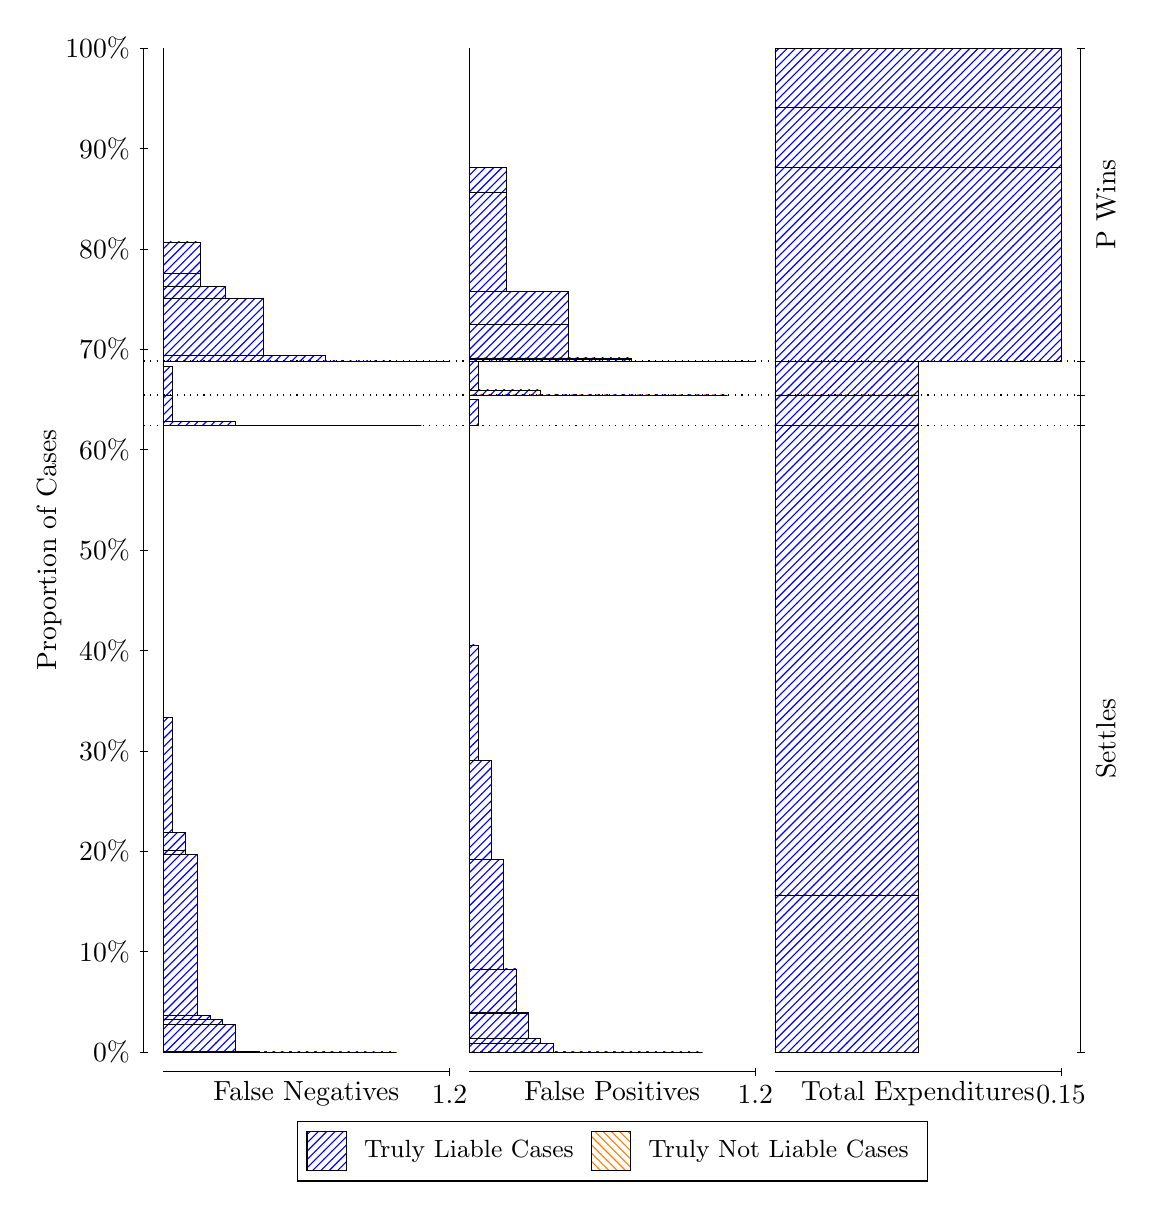
\begin{tikzpicture}
\draw[black, very thin] (1.5,1.75) -- (1.5,14.5);
\node[rotate=90, anchor=center] at (0.3, 8.125) {Proportion of Cases};
\draw[black, very thin] (1.45,1.75) -- (1.55,1.75);
\node[anchor=east] at (1.45, 1.75) {0\%};
\draw[black, very thin] (1.45,3.025) -- (1.55,3.025);
\node[anchor=east] at (1.45, 3.025) {10\%};
\draw[black, very thin] (1.45,4.3) -- (1.55,4.3);
\node[anchor=east] at (1.45, 4.3) {20\%};
\draw[black, very thin] (1.45,5.575) -- (1.55,5.575);
\node[anchor=east] at (1.45, 5.575) {30\%};
\draw[black, very thin] (1.45,6.85) -- (1.55,6.85);
\node[anchor=east] at (1.45, 6.85) {40\%};
\draw[black, very thin] (1.45,8.125) -- (1.55,8.125);
\node[anchor=east] at (1.45, 8.125) {50\%};
\draw[black, very thin] (1.45,9.4) -- (1.55,9.4);
\node[anchor=east] at (1.45, 9.4) {60\%};
\draw[black, very thin] (1.45,10.675) -- (1.55,10.675);
\node[anchor=east] at (1.45, 10.675) {70\%};
\draw[black, very thin] (1.45,11.95) -- (1.55,11.95);
\node[anchor=east] at (1.45, 11.95) {80\%};
\draw[black, very thin] (1.45,13.225) -- (1.55,13.225);
\node[anchor=east] at (1.45, 13.225) {90\%};
\draw[black, very thin] (1.45,14.5) -- (1.55,14.5);
\node[anchor=east] at (1.45, 14.5) {100\%};

\draw[black, very thin] (13.4,1.75) -- (13.4,14.5);
\draw[black, very thin] (13.35,1.75) -- (13.45,1.75);
\node[anchor=west] at (13.35, 1.75) {};
\draw[black, very thin] (13.35,9.7055) -- (13.45,9.7055);
\node[anchor=west] at (13.35, 9.7055) {};
\draw[black, very thin] (13.35,10.094) -- (13.45,10.094);
\node[anchor=west] at (13.35, 10.094) {};
\draw[black, very thin] (13.35,10.525) -- (13.45,10.525);
\node[anchor=west] at (13.35, 10.525) {};
\draw[black, very thin] (13.35,14.5) -- (13.45,14.5);
\node[anchor=west] at (13.35, 14.5) {};

\draw[black, very thin, pattern color=blue, pattern=north east lines] (1.75,1.75) rectangle (4.712,1.75);
\draw[black, very thin, pattern color=blue, pattern=north east lines] (1.75,1.75) rectangle (4.396,1.75);
\draw[black, very thin, pattern color=blue, pattern=north east lines] (1.75,1.75) rectangle (4.0801,1.75);
\draw[black, very thin, pattern color=blue, pattern=north east lines] (1.75,1.75) rectangle (3.9221,1.75);
\draw[black, very thin, pattern color=blue, pattern=north east lines] (1.75,1.75) rectangle (3.7641,1.75);
\draw[black, very thin, pattern color=blue, pattern=north east lines] (1.75,1.75) rectangle (3.6062,1.75);
\draw[black, very thin, pattern color=blue, pattern=north east lines] (1.75,1.75) rectangle (3.4482,1.7509);
\draw[black, very thin, pattern color=blue, pattern=north east lines] (1.75,1.7509) rectangle (3.2902,1.751);
\draw[black, very thin, pattern color=blue, pattern=north east lines] (1.75,1.751) rectangle (3.1322,1.7511);
\draw[black, very thin, pattern color=blue, pattern=north east lines] (1.75,1.7511) rectangle (2.9743,1.7511);
\draw[black, very thin, pattern color=blue, pattern=north east lines] (1.75,1.7511) rectangle (2.9743,1.754);
\draw[black, very thin, pattern color=blue, pattern=north east lines] (1.75,1.754) rectangle (2.8163,1.7572);
\draw[black, very thin, pattern color=blue, pattern=north east lines] (1.75,1.7572) rectangle (2.6583,2.098);
\draw[black, very thin, pattern color=blue, pattern=north east lines] (1.75,2.098) rectangle (2.5004,2.1635);
\draw[black, very thin, pattern color=blue, pattern=north east lines] (1.75,2.1635) rectangle (2.5004,2.1635);
\draw[black, very thin, pattern color=blue, pattern=north east lines] (1.75,2.1635) rectangle (2.3424,2.2195);
\draw[black, very thin, pattern color=blue, pattern=north east lines] (1.75,2.2195) rectangle (2.1844,2.2195);
\draw[black, very thin, pattern color=blue, pattern=north east lines] (1.75,2.2195) rectangle (2.1844,4.2569);
\draw[black, very thin, pattern color=blue, pattern=north east lines] (1.75,4.2569) rectangle (2.0264,4.309);
\draw[black, very thin, pattern color=blue, pattern=north east lines] (1.75,4.309) rectangle (2.0264,4.5369);
\draw[black, very thin, pattern color=blue, pattern=north east lines] (1.75,4.5369) rectangle (1.8685,5.9995);
\draw[black, very thin, pattern color=orange, pattern=north west lines] (1.75,5.9995) rectangle (1.75,5.9995);
\draw[black, very thin, pattern color=blue, pattern=north east lines] (1.75,5.9995) rectangle (1.75,9.7055);
\draw[black, very thin, pattern color=blue, pattern=north east lines] (1.75,9.7055) rectangle (5.0279,9.7055);
\draw[black, very thin, pattern color=blue, pattern=north east lines] (1.75,9.7055) rectangle (4.238,9.7055);
\draw[black, very thin, pattern color=blue, pattern=north east lines] (1.75,9.7055) rectangle (3.4482,9.7058);
\draw[black, very thin, pattern color=blue, pattern=north east lines] (1.75,9.7058) rectangle (2.6583,9.7577);
\draw[black, very thin, pattern color=blue, pattern=north east lines] (1.75,9.7577) rectangle (1.8685,10.094);
\draw[black, very thin, pattern color=orange, pattern=north west lines] (1.75,10.094) rectangle (1.75,10.094);
\draw[black, very thin, pattern color=blue, pattern=north east lines] (1.75,10.094) rectangle (1.8685,10.459);
\draw[black, very thin, pattern color=orange, pattern=north west lines] (1.75,10.459) rectangle (1.75,10.459);
\draw[black, very thin, pattern color=blue, pattern=north east lines] (1.75,10.459) rectangle (1.75,10.525);
\draw[black, very thin, pattern color=blue, pattern=north east lines] (1.75,10.525) rectangle (5.3833,10.525);
\draw[black, very thin, pattern color=blue, pattern=north east lines] (1.75,10.525) rectangle (4.5935,10.526);
\draw[black, very thin, pattern color=blue, pattern=north east lines] (1.75,10.526) rectangle (4.1196,10.526);
\draw[black, very thin, pattern color=blue, pattern=north east lines] (1.75,10.526) rectangle (3.8036,10.597);
\draw[black, very thin, pattern color=blue, pattern=north east lines] (1.75,10.597) rectangle (3.3297,10.597);
\draw[black, very thin, pattern color=blue, pattern=north east lines] (1.75,10.597) rectangle (3.0138,11.321);
\draw[black, very thin, pattern color=blue, pattern=north east lines] (1.75,11.321) rectangle (2.5399,11.47);
\draw[black, very thin, pattern color=blue, pattern=north east lines] (1.75,11.47) rectangle (2.2239,11.639);
\draw[black, very thin, pattern color=blue, pattern=north east lines] (1.75,11.639) rectangle (2.2239,12.038);
\draw[black, very thin, pattern color=orange, pattern=north west lines] (1.75,12.038) rectangle (1.75,12.038);
\draw[black, very thin, pattern color=blue, pattern=north east lines] (1.75,12.038) rectangle (1.75,14.5);
\draw[black, very thin, pattern color=orange, pattern=north west lines] (5.6333,1.75) rectangle (8.5953,1.75);
\draw[black, very thin, pattern color=blue, pattern=north east lines] (5.6333,1.75) rectangle (8.5953,1.75);
\draw[black, very thin, pattern color=orange, pattern=north west lines] (5.6333,1.75) rectangle (8.2793,1.75);
\draw[black, very thin, pattern color=blue, pattern=north east lines] (5.6333,1.75) rectangle (8.2793,1.75);
\draw[black, very thin, pattern color=orange, pattern=north west lines] (5.6333,1.75) rectangle (7.9634,1.75);
\draw[black, very thin, pattern color=blue, pattern=north east lines] (5.6333,1.75) rectangle (7.9634,1.75);
\draw[black, very thin, pattern color=blue, pattern=north east lines] (5.6333,1.75) rectangle (7.8054,1.75);
\draw[black, very thin, pattern color=orange, pattern=north west lines] (5.6333,1.75) rectangle (7.6475,1.75);
\draw[black, very thin, pattern color=blue, pattern=north east lines] (5.6333,1.75) rectangle (7.6475,1.75);
\draw[black, very thin, pattern color=blue, pattern=north east lines] (5.6333,1.75) rectangle (7.4895,1.75);
\draw[black, very thin, pattern color=orange, pattern=north west lines] (5.6333,1.75) rectangle (7.3315,1.75);
\draw[black, very thin, pattern color=blue, pattern=north east lines] (5.6333,1.75) rectangle (7.3315,1.7501);
\draw[black, very thin, pattern color=blue, pattern=north east lines] (5.6333,1.7501) rectangle (7.1736,1.7501);
\draw[black, very thin, pattern color=orange, pattern=north west lines] (5.6333,1.7501) rectangle (7.0156,1.7501);
\draw[black, very thin, pattern color=blue, pattern=north east lines] (5.6333,1.7501) rectangle (7.0156,1.7515);
\draw[black, very thin, pattern color=orange, pattern=north west lines] (5.6333,1.7515) rectangle (7.0156,1.7515);
\draw[black, very thin, pattern color=blue, pattern=north east lines] (5.6333,1.7515) rectangle (7.0156,1.7515);
\draw[black, very thin, pattern color=blue, pattern=north east lines] (5.6333,1.7515) rectangle (6.8576,1.7515);
\draw[black, very thin, pattern color=blue, pattern=north east lines] (5.6333,1.7515) rectangle (6.6996,1.7515);
\draw[black, very thin, pattern color=orange, pattern=north west lines] (5.6333,1.7515) rectangle (6.6996,1.7515);
\draw[black, very thin, pattern color=blue, pattern=north east lines] (5.6333,1.7515) rectangle (6.6996,1.8591);
\draw[black, very thin, pattern color=blue, pattern=north east lines] (5.6333,1.8591) rectangle (6.5417,1.9256);
\draw[black, very thin, pattern color=orange, pattern=north west lines] (5.6333,1.9256) rectangle (6.3837,1.9256);
\draw[black, very thin, pattern color=blue, pattern=north east lines] (5.6333,1.9256) rectangle (6.3837,2.2467);
\draw[black, very thin, pattern color=blue, pattern=north east lines] (5.6333,2.2467) rectangle (6.3837,2.2486);
\draw[black, very thin, pattern color=blue, pattern=north east lines] (5.6333,2.2486) rectangle (6.2257,2.8062);
\draw[black, very thin, pattern color=blue, pattern=north east lines] (5.6333,2.8062) rectangle (6.2257,2.8062);
\draw[black, very thin, pattern color=orange, pattern=north west lines] (5.6333,2.8062) rectangle (6.0678,2.8062);
\draw[black, very thin, pattern color=blue, pattern=north east lines] (5.6333,2.8062) rectangle (6.0678,4.1996);
\draw[black, very thin, pattern color=blue, pattern=north east lines] (5.6333,4.1996) rectangle (6.0678,4.2001);
\draw[black, very thin, pattern color=blue, pattern=north east lines] (5.6333,4.2001) rectangle (5.9098,4.2001);
\draw[black, very thin, pattern color=blue, pattern=north east lines] (5.6333,4.2001) rectangle (5.9098,5.456);
\draw[black, very thin, pattern color=blue, pattern=north east lines] (5.6333,5.456) rectangle (5.7518,6.9186);
\draw[black, very thin, pattern color=blue, pattern=north east lines] (5.6333,6.9186) rectangle (5.6333,9.7055);
\draw[black, very thin, pattern color=orange, pattern=north west lines] (5.6333,9.7055) rectangle (5.7518,9.7055);
\draw[black, very thin, pattern color=blue, pattern=north east lines] (5.6333,9.7055) rectangle (5.7518,10.041);
\draw[black, very thin, pattern color=blue, pattern=north east lines] (5.6333,10.041) rectangle (5.6333,10.094);
\draw[black, very thin, pattern color=orange, pattern=north west lines] (5.6333,10.094) rectangle (8.9112,10.094);
\draw[black, very thin, pattern color=blue, pattern=north east lines] (5.6333,10.094) rectangle (8.9112,10.094);
\draw[black, very thin, pattern color=blue, pattern=north east lines] (5.6333,10.094) rectangle (8.1214,10.094);
\draw[black, very thin, pattern color=blue, pattern=north east lines] (5.6333,10.094) rectangle (7.3315,10.094);
\draw[black, very thin, pattern color=blue, pattern=north east lines] (5.6333,10.094) rectangle (6.5417,10.159);
\draw[black, very thin, pattern color=blue, pattern=north east lines] (5.6333,10.159) rectangle (5.7518,10.525);
\draw[black, very thin, pattern color=orange, pattern=north west lines] (5.6333,10.525) rectangle (9.2667,10.525);
\draw[black, very thin, pattern color=blue, pattern=north east lines] (5.6333,10.525) rectangle (9.2667,10.525);
\draw[black, very thin, pattern color=orange, pattern=north west lines] (5.6333,10.525) rectangle (8.4768,10.525);
\draw[black, very thin, pattern color=blue, pattern=north east lines] (5.6333,10.525) rectangle (8.4768,10.525);
\draw[black, very thin, pattern color=blue, pattern=north east lines] (5.6333,10.525) rectangle (8.4768,10.525);
\draw[black, very thin, pattern color=orange, pattern=north west lines] (5.6333,10.525) rectangle (7.687,10.525);
\draw[black, very thin, pattern color=blue, pattern=north east lines] (5.6333,10.525) rectangle (7.687,10.551);
\draw[black, very thin, pattern color=blue, pattern=north east lines] (5.6333,10.551) rectangle (7.687,10.566);
\draw[black, very thin, pattern color=orange, pattern=north west lines] (5.6333,10.566) rectangle (7.213,10.566);
\draw[black, very thin, pattern color=blue, pattern=north east lines] (5.6333,10.566) rectangle (7.213,10.566);
\draw[black, very thin, pattern color=orange, pattern=north west lines] (5.6333,10.566) rectangle (6.8971,10.566);
\draw[black, very thin, pattern color=blue, pattern=north east lines] (5.6333,10.566) rectangle (6.8971,10.987);
\draw[black, very thin, pattern color=blue, pattern=north east lines] (5.6333,10.987) rectangle (6.8971,11.412);
\draw[black, very thin, pattern color=orange, pattern=north west lines] (5.6333,11.412) rectangle (6.4232,11.412);
\draw[black, very thin, pattern color=blue, pattern=north east lines] (5.6333,11.412) rectangle (6.4232,11.413);
\draw[black, very thin, pattern color=blue, pattern=north east lines] (5.6333,11.413) rectangle (6.1072,12.669);
\draw[black, very thin, pattern color=blue, pattern=north east lines] (5.6333,12.669) rectangle (6.1072,12.986);
\draw[black, very thin, pattern color=orange, pattern=north west lines] (5.6333,12.986) rectangle (5.6333,12.986);
\draw[black, very thin, pattern color=blue, pattern=north east lines] (5.6333,12.986) rectangle (5.6333,14.5);
\draw[black, very thin, pattern color=orange, pattern=north west lines] (9.5167,1.75) rectangle (11.333,1.75);
\draw[black, very thin, pattern color=blue, pattern=north east lines] (9.5167,1.75) rectangle (11.333,3.7452);
\draw[black, very thin, pattern color=orange, pattern=north west lines] (9.5167,3.7452) rectangle (11.333,3.7452);
\draw[black, very thin, pattern color=blue, pattern=north east lines] (9.5167,3.7452) rectangle (11.333,9.7055);
\draw[black, very thin, pattern color=orange, pattern=north west lines] (9.5167,9.7055) rectangle (11.333,9.7055);
\draw[black, very thin, pattern color=blue, pattern=north east lines] (9.5167,9.7055) rectangle (11.333,10.094);
\draw[black, very thin, pattern color=orange, pattern=north west lines] (9.5167,10.094) rectangle (11.333,10.094);
\draw[black, very thin, pattern color=blue, pattern=north east lines] (9.5167,10.094) rectangle (11.333,10.525);
\draw[black, very thin, pattern color=orange, pattern=north west lines] (9.5167,10.525) rectangle (13.15,10.525);
\draw[black, very thin, pattern color=blue, pattern=north east lines] (9.5167,10.525) rectangle (13.15,12.984);
\draw[black, very thin, pattern color=orange, pattern=north west lines] (9.5167,12.984) rectangle (13.15,12.984);
\draw[black, very thin, pattern color=blue, pattern=north east lines] (9.5167,12.984) rectangle (13.15,13.742);
\draw[black, very thin, pattern color=orange, pattern=north west lines] (9.5167,13.742) rectangle (13.15,13.742);
\draw[black, very thin, pattern color=blue, pattern=north east lines] (9.5167,13.742) rectangle (13.15,14.5);
\draw[black, dotted] (1.5,9.7055) -- (13.4,9.7055);
\draw[black, dotted] (1.5,10.094) -- (13.4,10.094);
\draw[black, dotted] (1.5,10.525) -- (13.4,10.525);
\draw[black, very thin] (1.75,1.5) -- (5.3833,1.5);
\node[anchor=north] at (3.5667, 1.5) {False Negatives};
\draw[black, very thin] (5.3833,1.45) -- (5.3833,1.55);
\node[anchor=north] at (5.3833, 1.45) {1.2};

\draw[black, very thin] (5.6333,1.5) -- (9.2667,1.5);
\node[anchor=north] at (7.45, 1.5) {False Positives};
\draw[black, very thin] (9.2667,1.45) -- (9.2667,1.55);
\node[anchor=north] at (9.2667, 1.45) {1.2};

\draw[black, very thin] (9.5167,1.5) -- (13.15,1.5);
\node[anchor=north] at (11.333, 1.5) {Total Expenditures};
\draw[black, very thin] (13.15,1.45) -- (13.15,1.55);
\node[anchor=north] at (13.15, 1.45) {0.15};

\node[black, centered, rotate=90] at (13.72, 5.7277) {Settles};


\node[black, centered, rotate=90] at (13.72, 12.512) {P Wins};

\draw (7.449999999999999,1.5) node[draw=none] (baseCoordinate) {};
\begin{scope}[align=center]
        \matrix[scale=0.5, draw=black, below=0.5cm of baseCoordinate, nodes={draw}, column sep=0.1cm]{
            \node[rectangle, draw, minimum width=0.5cm, minimum height=0.5cm, pattern=north east lines, pattern color=blue] {}; &
            \node[draw=none, font=\small] (B) {Truly Liable Cases}; &
            \node[rectangle, draw, minimum width=0.5cm, minimum height=0.5cm, pattern=north west lines, pattern color=orange] {}; &
            \node[draw=none, font=\small] (B) {Truly Not Liable Cases}; \\
            };
\end{scope}

\end{tikzpicture}
\end{document}